\documentclass{standalone}
\usepackage[T1]{fontenc}\usepackage{tikz}
\usepackage{amsmath, amsfonts}
\usetikzlibrary{arrows, shapes.geometric, calc, positioning, decorations.pathreplacing}

\tikzstyle{chainName} = [rectangle, rounded corners, minimum width=3cm, minimum height=1cm, text centered, draw=black]
\tikzstyle{block} = [rectangle, rounded corners, minimum width=1cm, minimum height=1cm, draw=black]
\tikzstyle{dots} = [inner sep=0pt, text height=10pt]
\tikzstyle{arrowParent} = [thick, ->, -to, shorten >= 2pt, shorten <= 2pt]
\tikzstyle{arrowRefl} = [dashed, ->, -to, shorten >= 2pt, shorten <= 2pt]
\tikzstyle{ethBrace} = [decorate, decoration={brace,amplitude=10pt,mirror}, xshift=4pt, sloped, rotate=180]

\begin{document}
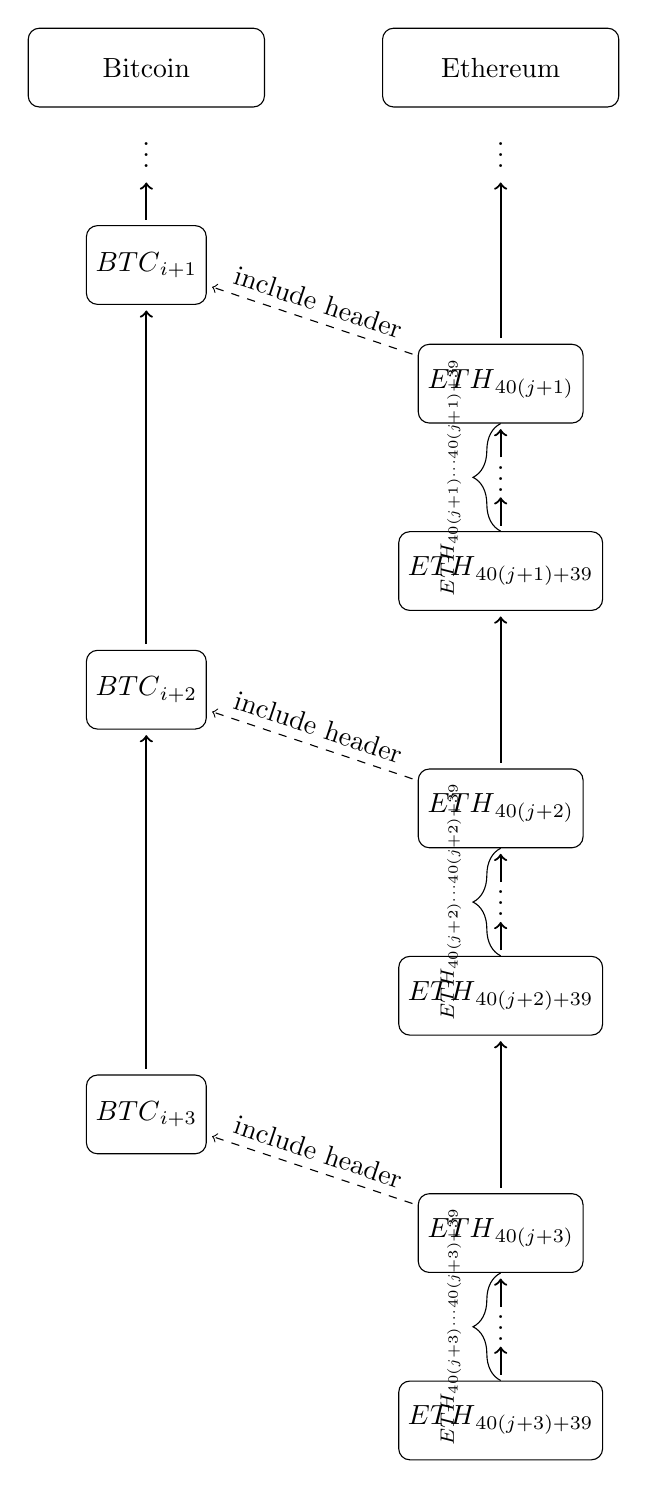
\begin{tikzpicture}[node distance=1cm]

    \node (btcChain) [chainName] {Bitcoin};
    \node (ethChain) [chainName, right of=btcChain, xshift=3.5cm] {Ethereum};

    \foreach \net/\oNet in {btc/eth,eth/btc} {
        \node (\net Dots) [below of=\net Chain, yshift=0cm] {$\vdots$};
    }

    \foreach \x in {1,...,3} {
        \pgfmathtruncatemacro\r{round(\x-1)}

        % bitcoin

        \ifnum 1=\x
        \xdef\ys{0}
        \xdef\prevNode{btcDots}
        \xdef\oPrev{ethDots}
        \else
        % \xdef\ys{-1cm}
        \xdef\prevNode{btc\r}
        \xdef\oPrev{ethE\r}
        \fi

        \node (btc\x) [block, below = of \prevNode |- \oPrev, yshift=\ys] {$\MakeUppercase{btc}_{i+\x}$};
        \draw [arrowParent] (btc\x) -- (\prevNode);

        % ethereum

        \xdef\ys{0}

        \ifnum 1=\x
        \xdef\prevNode{ethDots}
        \xdef\oPrev{btc1}
        \else
        \xdef\prevNode{ethE\r}
        \xdef\oPrev{btc\x}
        \fi

        \node (ethS\x) [block, below = of \prevNode |- \oPrev, yshift=\ys] {$\MakeUppercase{eth}_{40(j+\x)}$};
        \draw [arrowParent] (ethS\x) -- (\prevNode);

        \node (ethDots\x) [dots, below = of ethS\x, yshift=0.5cm] {\vdots};
        \draw [arrowParent] (ethDots\x) -- (ethS\x);

        \node (ethE\x) [block, below = of ethDots\x, yshift=0.5cm] {$\MakeUppercase{eth}_{40(j+\x) + 39}$};
        \draw [arrowParent] (ethE\x) -- (ethDots\x);

        \draw [arrowRefl] (ethS\x) -- node[anchor=center, above, sloped] {include header} (\oPrev);

        \draw [ethBrace] (ethS\x) -- (ethE\x) node[black, midway, yshift=18pt] {\scriptsize{$ETH_{40(j+\x) \cdots 40(j+\x)+39}$}};
    }

\end{tikzpicture}
\end{document}
